%Experimental Results and Analysis – in this section, you should show the quantitative results – charts and tables. Analyze the results by explaining and highlighting what is important on them in terms of your goals and what is bad. You should explain the strange results too.

%V ďalšej časti prezentujte vlastný prínos a vlastné výsledky porovnajte s výsledkami iných. Charakterizujte použité metódy.
%Vyhýbajte sa používaniu žargónu.
%Používajte starú múdrosť: 1 obrázok je viac než 1000 slov.

\subsection{Complex binary vector associations} 
\label{sec:results-k3}

TODO Explain how it was measured (runs, epochs, stopping) \\
TODO Explain / Make up hypotheses why it behaves as measured (Future work). \\

(\ref{sec:datasets-k3}) 


\subsubsection{Two learning rates} 
\label{sec:tlr-k3}
TODO write here sth 

%Main purpose of this dataset is to test different hidden sizes 
%======== (4D) L1 x L2 x patSuccF x hidden size =========
%======== (4D) L1 x L2 x epochs x hidden size =========

\begin{figure}[H]
  \centering
  Hidden size = 3 \\
  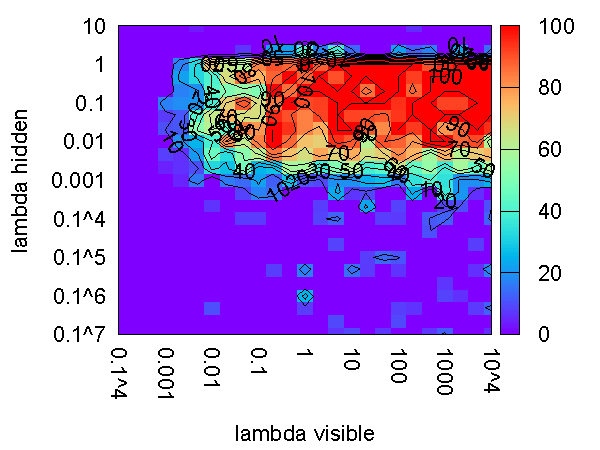
\includegraphics[width=0.49\textwidth]{img/k3/tlr-3-success.pdf} 
  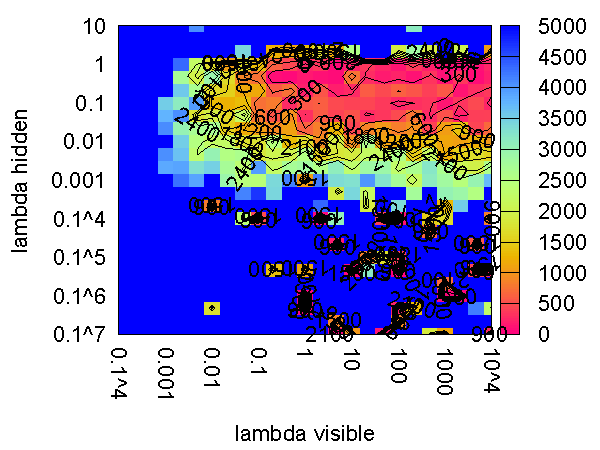
\includegraphics[width=0.49\textwidth]{img/k3/tlr-3-epoch.pdf}   
  Hidden size = 4 \\
  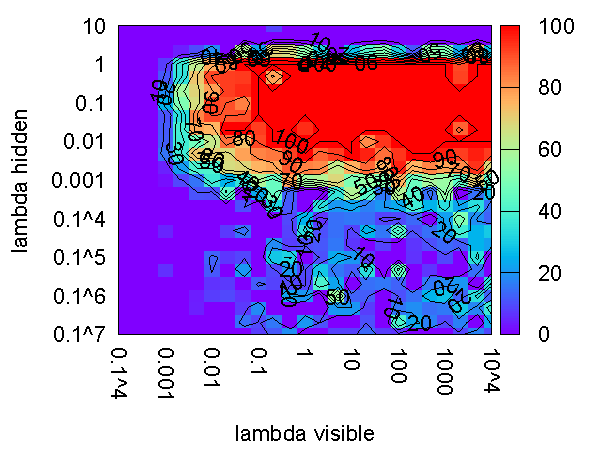
\includegraphics[width=0.49\textwidth]{img/k3/tlr-4-success.pdf} 
  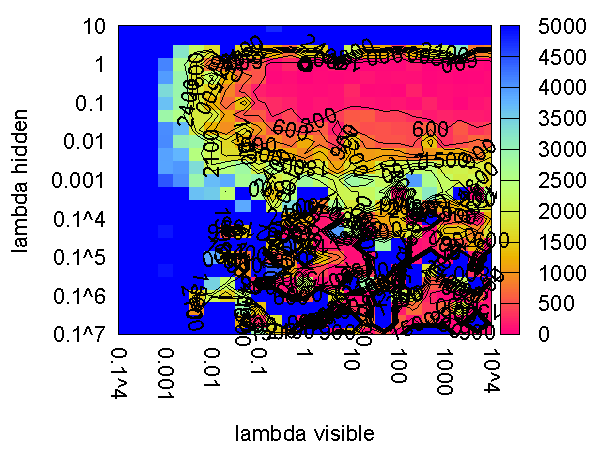
\includegraphics[width=0.49\textwidth]{img/k3/tlr-4-epoch.pdf}   
  Hidden size = 5 \\
  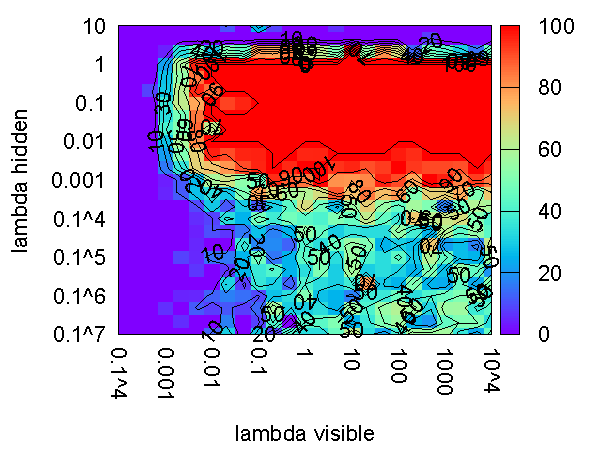
\includegraphics[width=0.49\textwidth]{img/k3/tlr-5-success.pdf}   
  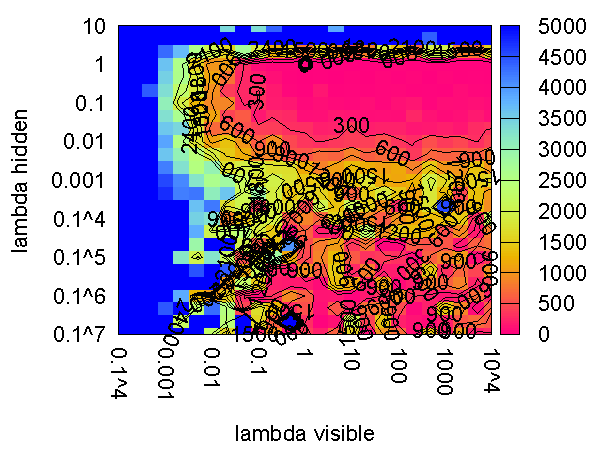
\includegraphics[width=0.49\textwidth]{img/k3/tlr-5-epoch.pdf}  
  Hidden size = 7 \\
  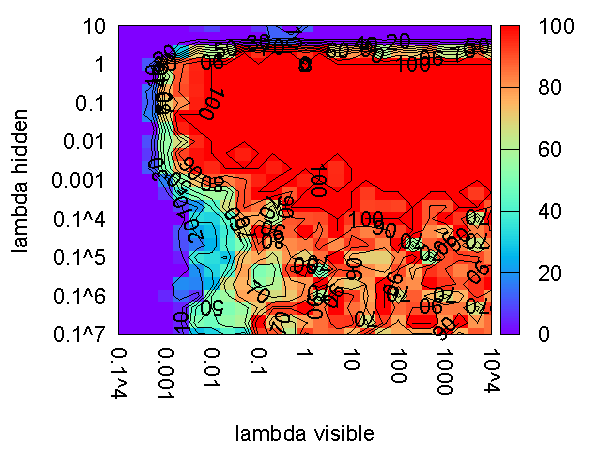
\includegraphics[width=0.49\textwidth]{img/k3/tlr-7-success.pdf} 
  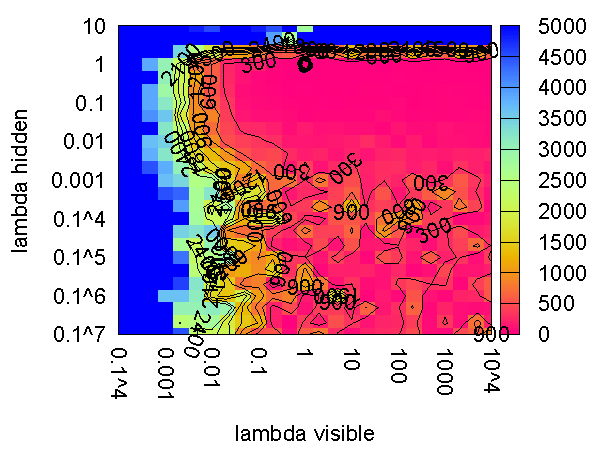
\includegraphics[width=0.49\textwidth]{img/k3/tlr-7-epoch.pdf}    
  \caption{TLR performance on the \emph{CBVA} task with different hidden sizes.}
  \label{fig:results-tlr-k3-success}
\end{figure}

%======== (3D) best TLR on ALL_SUCC x epoch (std-dev) x hidden size ==========
\begin{figure}[H]
  \centering
  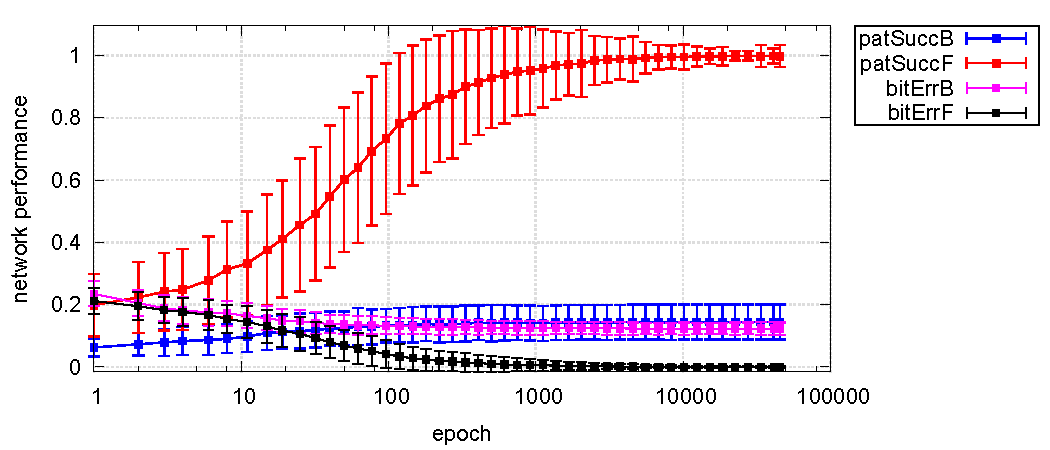
\includegraphics[width=0.8\textwidth]{img/tlr-k3-3-best-perf.pdf}   
  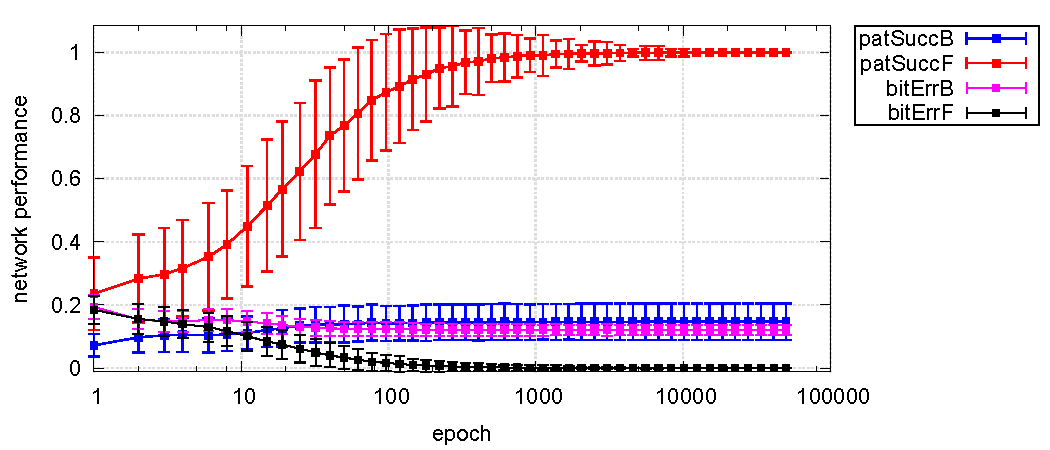
\includegraphics[width=0.8\textwidth]{img/tlr-k3-3-best-can.pdf}      
  \caption{TLR success timeline for the \emph{CBVA} task with $\lambda_h=0.1$ and $\lambda_v=100$. Top without candidate selection and bottom with candidates selection. }
  \label{fig:results-tlr-k3-epoch} 
\end{figure}

\subsubsection{Comparison} 
\label{sec:results-cmp-k3} 

%===== TODO table: best parameter setting networks with hidden.size= constant (success, epoch, stddev) / model \\

\begin{table}[H] 
  \centering
    \begin{tabular}{|l|l|l|l|l|}
    \hline
    Algorithm (section)&$\lambda_h$&$\lambda_v$&$patSucc^F$ &Epochs\\ %&SEM(success) \\
    \hline
    GR~(\ref{sec:models-generec}) &1.0 &1.0 &95&191.24\\ %&28\\
    \hline
    GR TLR~(\ref{sec:models-generec}) &3.0 &0.1 &97&156.52\\ %&28\\
    \hline
    BAL~(\ref{sec:models-bal})&0.5 &0.5 &100& 54\\ %&2.0e+08\\
    \hline
    BAL TLR~(\ref{sec:our-tlr})&1.0& 5.0 & 100& 64\\ %&1.52e+08\\
    \hline
    BAL TLR Can~(\ref{sec:sim-exp-candidates})& & & & \\ %&5,070,000\\ %TODO shit, wrong params 
    \hline 
    \end{tabular}
  \caption{Comparing performance of different models on the \emph{4-2-4 encoder} task with 3 hidden neurons.} 
  \label{tab:results-cmp-k3}
\end{table}

%SELECT lambda, lambda_ih, 100*AVG(success) AS 'suc', AVG(epoch) AS 'epc' FROM data WHERE epoch <> 0 GROUP BY lambda,lambda_ih ORDER BY suc ASC, epc DESC; 
%generec tlr
%0.3|1.0|95.0|181.68
%0.1|0.03|96.0|293.77
%0.1|1.0e-08|96.0|213.9
%0.3|0.0001|96.0|191.85
%0.1|3.0|97.0|156.52

%generec pure 
%0.01|0.01|85.0|960.62
%0.03|0.03|93.0|433.5
%0.1|0.1|95.0|260.0
%0.3|0.3|95.0|202.93
%1.0|1.0|95.0|191.24


%tlr pure 
%2.0|0.5|100.0|98.7777777777778
%2000.0|1.0|100.0|86.48
%5000.0|0.5|100.0|77.1428571428571
%5.0|1.0|100.0|64.0
%0.5|0.5|100.0|54.0

%tlr candidate 


\subsubsection{GeneRec} 
TODO write here sthh

\begin{figure}[H]
  \centering
  Hidden size = 3 \\
  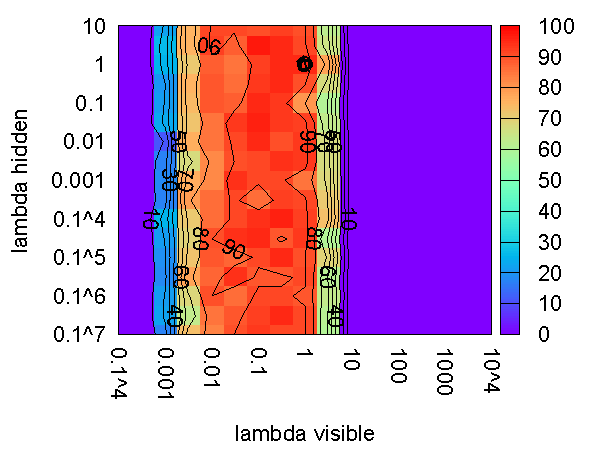
\includegraphics[width=0.49\textwidth]{img/k3/generec-3-success.pdf} 
  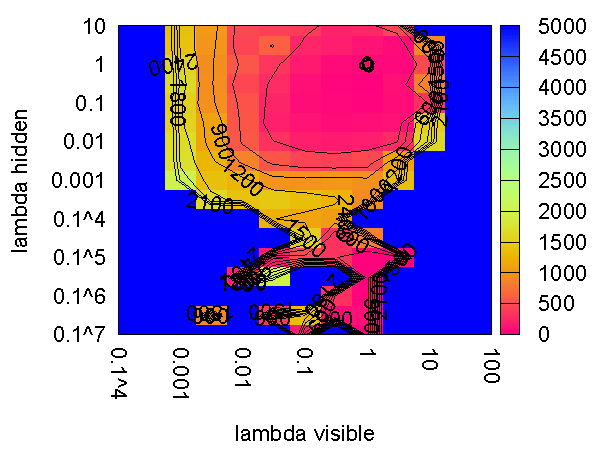
\includegraphics[width=0.49\textwidth]{img/k3/generec-3-epoch.pdf}   
%  Hidden size = 4 \\
%  \includegraphics[width=0.49\textwidth]{img/k3/generec-4-success.pdf} 
%  \includegraphics[width=0.49\textwidth]{img/k3/generec-4-epoch.pdf}   
  Hidden size = 5 \\
  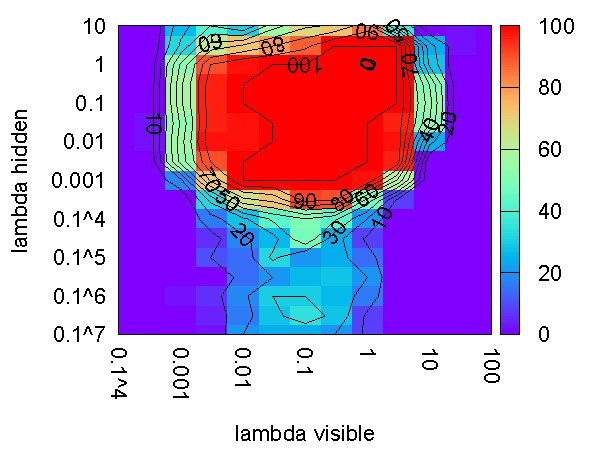
\includegraphics[width=0.49\textwidth]{img/k3/generec-5-success.pdf} 
  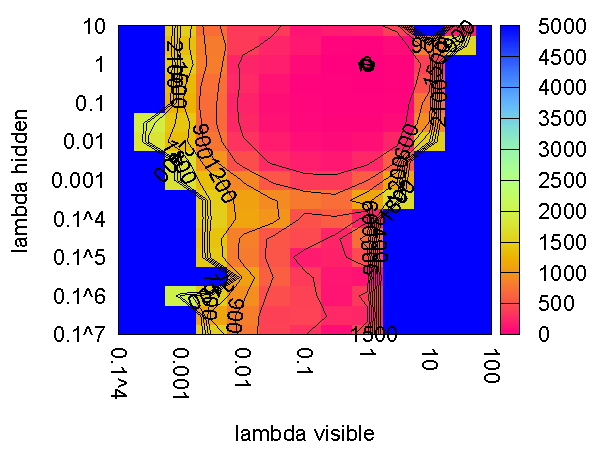
\includegraphics[width=0.49\textwidth]{img/k3/generec-5-epoch.pdf}  
%  Hidden size = 7 \\
%  \includegraphics[width=0.49\textwidth]{img/k3/generec-7-success.pdf} 
%  \includegraphics[width=0.49\textwidth]{img/k3/generec-7-epoch.pdf}    
  \caption{\emph{GeneRec} performance on the \emph{CBVA} task with different hidden sizes. For greater hidden sizes the results were very similar to the results with hidden size 5.}
  \label{fig:results-generec-k3-success}
\end{figure}

